\documentclass[hyperref={pdfpagelabels=false}]{beamer}
\usepackage{lmodern}
\usepackage[cp1251]{inputenc}
\usepackage[russian]{babel}
\usepackage{amsmath,mathrsfs,mathtext}
\usepackage{graphicx, epsfig}
\usepackage{subfig}
\usepackage{floatflt}
\usepackage{epic,ecltree}
\usepackage{mathtext}
\usepackage{fancybox}
\usepackage{fancyhdr}
\usepackage{enumerate}
\usepackage{epstopdf}
\usepackage{multicol}
\usepackage{ulem}
\usepackage{amsfonts}
\usepackage{array}
\usepackage{makecell}
\usepackage{colortbl}
\usepackage{hhline}
\usepackage{subfig}
\usepackage{epstopdf}
\usepackage{caption}
\usepackage[strict]{changepage}
\renewcommand{\thefigure}{\arabic{figure}}
\renewcommand{\thetable}{\arabic{table}}
\DeclareMathOperator*{\argmin}{arg\,min}

\captionsetup[figure]{labelformat=empty}

\usetheme{Frankfurt}
\definecolor{beamer@blendedblue}{RGB}{0, 50, 50}

\setbeamertemplate{footline}
{
  \leavevmode%
  \hbox{%
  \begin{beamercolorbox}[wd=.5\paperwidth,ht=2.25ex,dp=1ex,right]{author in head/foot}%
    \usebeamerfont{author in head/foot}\insertshortauthor\hspace{1em}
  \end{beamercolorbox}%
  \begin{beamercolorbox}[wd=.5\paperwidth,ht=2.25ex,dp=1ex,left]{title in head/foot}%
    \usebeamerfont{title in head/foot}\hspace{1em}\insertshorttitle
  \end{beamercolorbox}}%
  \vskip0pt%
}

\title[Image restoration] {Restoration of blurred noisy images}
\author[Projectors]{\large \\Anastasia Belozerova \\ Ekaterina Chuikova \\ Daria Fokina \\ Fedor Streltsov}

\institute[Skoltech]{Skolkovo Institute of Science and Technology
    \vspace{0.3cm} \\
	Courses: Optimization Methods, NLA }
\date{}
%------------------------------------------------------------------------------
\begin{document}
\begin{frame}
\titlepage
\end{frame} 
%------------------------------------------------------------------------------
\section{Introduction} 
\subsection{Project Proposal}
\begin{frame}
\frametitle{Project Proposal} 
\begin{block}{Task}
Given the observed blurry noisy image and blur matrix restore the initial image
\end{block}

\begin{block}{Applications}
\begin{itemize}
\item Micro science
\item Security 
\item Photography industry
\item Computer vision 
\end{itemize}

\end{block}

\end{frame}

%------------------------------------------------------------------------------
\subsection{Works}
\begin{frame}
\frametitle{Related Works} 
\begin{itemize}
\item A. Danielyan, V. Katkovnik, K. Egiazarian, BM3D frames and variational image deblurring, 2011.
\item N. P. Galatsanos, A.K. Katsaggelos, Methods for choosing the regularization parameter and estimating the noise variance in image restoration and their relation, 1992.
\item Lu Yuan, Jian Sun, Long Quan, Heung-Yeung Shum, Progressive Inter-scale and Intra-scale Non-blind Image Deconvolution.

\end{itemize}
\end{frame}
%------------------------------------------------------------------------------

\subsection{Problem Statement}
\begin{frame}
\frametitle{Problem Statement} 

\begin{block}{Notation}
Let $z:3 \times N^2$ be vector-reshaped observed image, \\
$A$ - blur matrix, $\sigma$ - derivation of additional noise, \\
$y: 3 \times N^2$ - initial image we are trying to restore, \\
$p(y)$ - penalty ('l1' and 'l2' are considered), $\tau$ - penalty parameter.
\end{block}

\begin{block}{Formulation}
\begin{align}
\hat y = \argmin_{y\in \mathbb{R}^{n^2}}  \left( \frac{1}{2\sigma} ||z - Ay ||_2^2 + \tau p(y) \right), \\
0 \leq \hat y_{ij} \leq 1, \forall i,j
\end{align}
\end{block}


\end{frame}
%------------------------------------------------------------------------------
\subsection{Data}
\begin{frame}
\frametitle{Preparing Data}

\begin{itemize}
\item Google photo of Skolkovo
\item Take gaussian filter
\item Create kernel
\item Reduce convolution to matvec operation
\item Add some noise
\end{itemize}

\begin{center}
\begin{figure}[h]
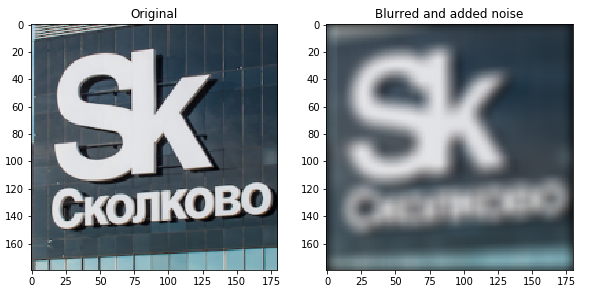
\includegraphics[scale=0.53]{filter.png}
\end{figure}
\end{center}

\end{frame}
%------------------------------------------------------------------------------
\section{Solution} 
\subsection{Methods}
\begin{frame}
\frametitle{Implemented Methods}

\begin{itemize}
\item cvxpy, lstsq, gurobi
\item Projected Gradient Descent, Fast Gradient
\item Proxi-Gradient
\item Newton method

\end{itemize}

\begin{block}{Variations}
\begin{itemize}
\item Regularizations
\item Kernels
\item Initializations
\end{itemize}
\end{block}
\end{frame}
%------------------------------------------------------------------------------
\subsection{CVXPY}
\begin{frame}
\frametitle{CVXPY. Various Kernels}

\begin{center}
\begin{figure}[h]
\begin{adjustwidth}{-0.2cm}{-0.5 cm}
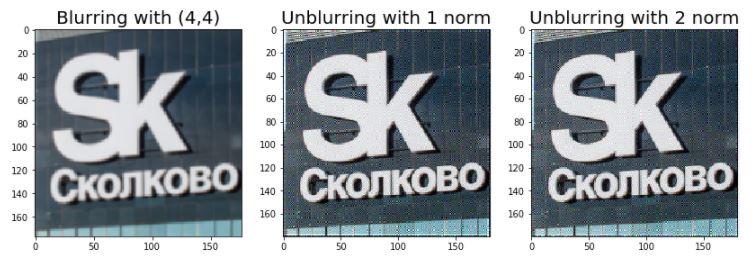
\includegraphics[scale=0.53]{4_4.jpg} \\
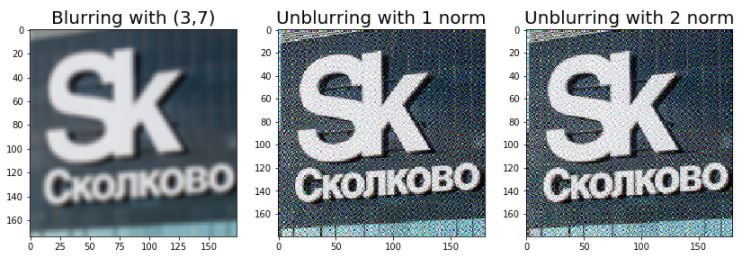
\includegraphics[scale=0.53]{3_7.jpg} \\
\end{adjustwidth}
\caption{.}
\end{figure}
\end{center}

\end{frame}
%------------------------------------------------------------------------------
\begin{frame}
\frametitle{CVXPY. Various Kernels}

\begin{center}
\begin{figure}[h]
\begin{adjustwidth}{-0.2cm}{-0.5 cm}
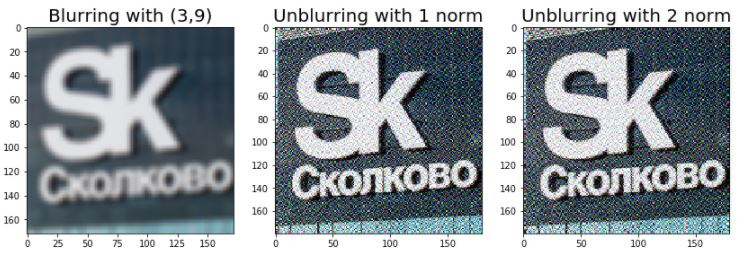
\includegraphics[scale=0.53]{3_9.jpg} \\
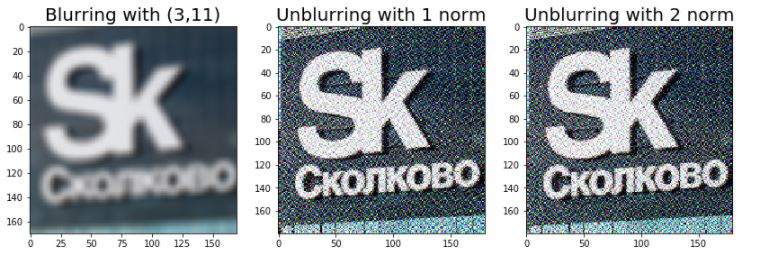
\includegraphics[scale=0.53]{3_11.jpg} \\
\end{adjustwidth}
\caption{.}
\end{figure}
\end{center}

\end{frame}
%------------------------------------------------------------------------------
\begin{frame}
\frametitle{CVXPY. Various Kernels}

\begin{center}
\begin{figure}[h]
\begin{adjustwidth}{-0.2cm}{-0.5 cm}
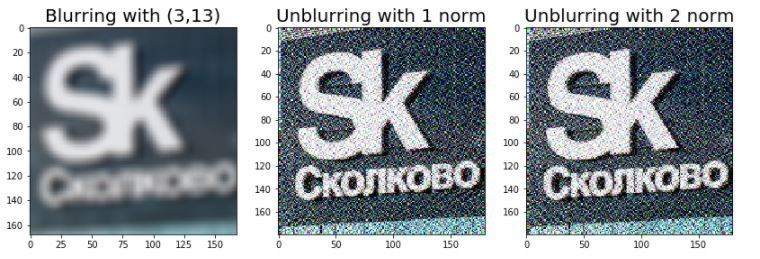
\includegraphics[scale=0.53]{3_13.jpg} \\
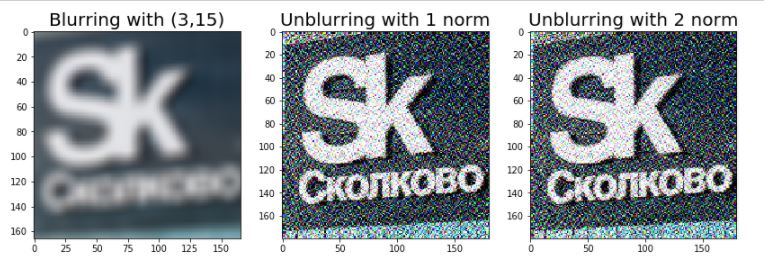
\includegraphics[scale=0.53]{3_15.jpg} \\
\end{adjustwidth}
\caption{.}
\end{figure}
\end{center}

\end{frame}
%------------------------------------------------------------------------------
\begin{frame}
\frametitle{CVXPY. Comparison}

\begin{center}
\begin{figure}[h]
\begin{adjustwidth}{-0.2cm}{-0.5 cm}
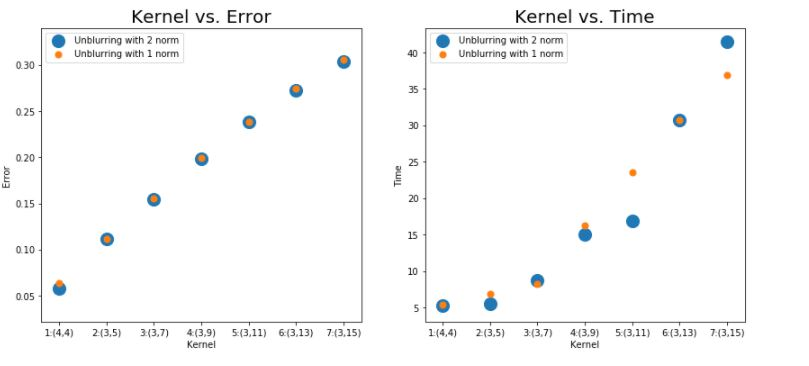
\includegraphics[scale=0.55]{Kern.jpg}
\end{adjustwidth}
\caption{.}
\end{figure}
\end{center}

\end{frame}
%------------------------------------------------------------------------------
\subsection{Gradient Descent}
\begin{frame}
\frametitle{Gradient Descent. Vanilla and Fast}

\begin{center}
\begin{figure}[h]
\begin{adjustwidth}{-0.5cm}{-0.5 cm}
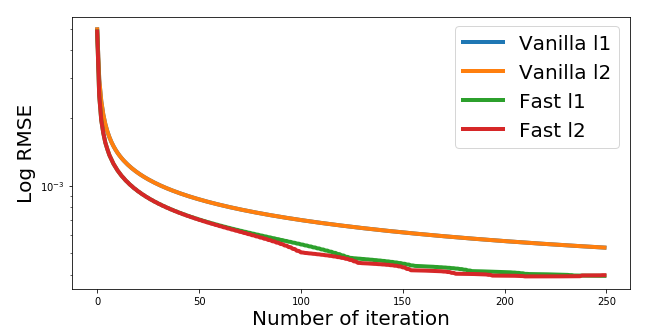
\includegraphics[scale=0.67]{van_fast.png}
\end{adjustwidth}
\caption{.}
\end{figure}
\end{center}

\end{frame}
%------------------------------------------------------------------------------
\begin{frame}
\frametitle{Fast Gradient. Different initializations}

\begin{center}
\begin{figure}[h]
\begin{adjustwidth}{-0.2cm}{-0.5 cm}
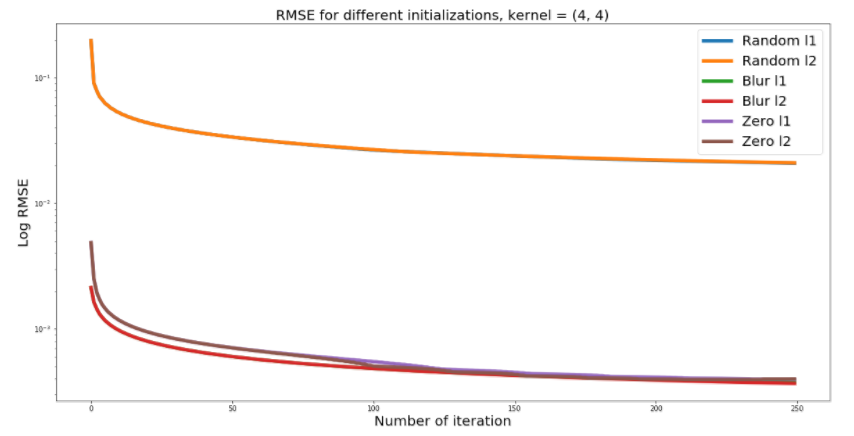
\includegraphics[scale=0.5]{grad_init.png}
\end{adjustwidth}
\caption{.}
\end{figure}
\end{center}

\end{frame}
%------------------------------------------------------------------------------
\begin{frame}
\frametitle{Fast Gradient. Different initializations}

\begin{center}
\begin{figure}[h]
\begin{adjustwidth}{-0.8cm}{-0.5 cm}
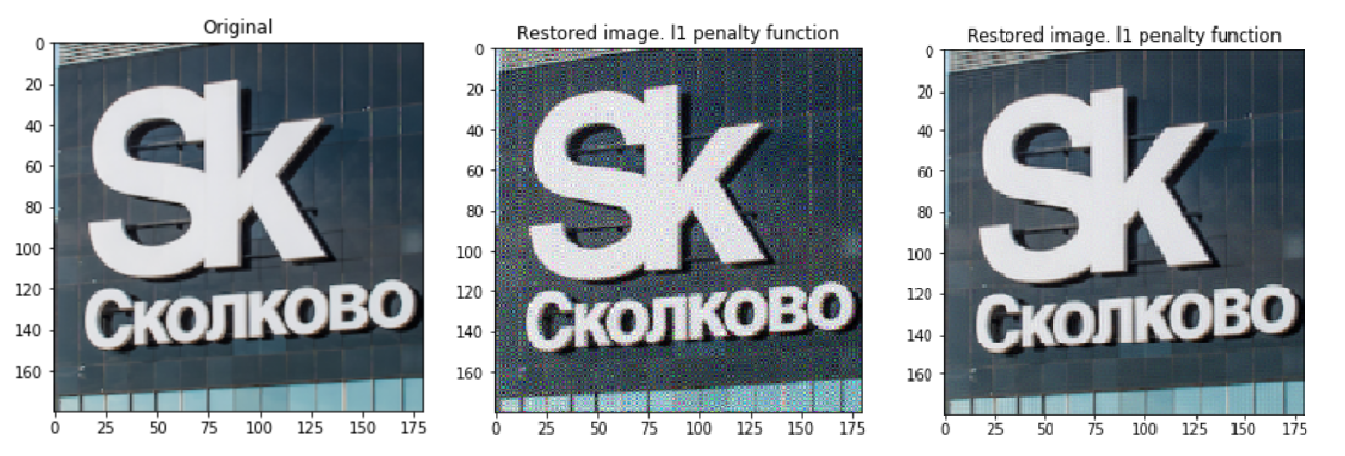
\includegraphics[scale=0.35]{methods.png}
\end{adjustwidth}
\caption{.}
\end{figure}
\end{center}

\end{frame}
%------------------------------------------------------------------------------
\begin{frame}
\frametitle{Comparison of two kernel's results}

\begin{center}
\begin{figure}[h]
\begin{adjustwidth}{-0.2cm}{-0.5 cm}
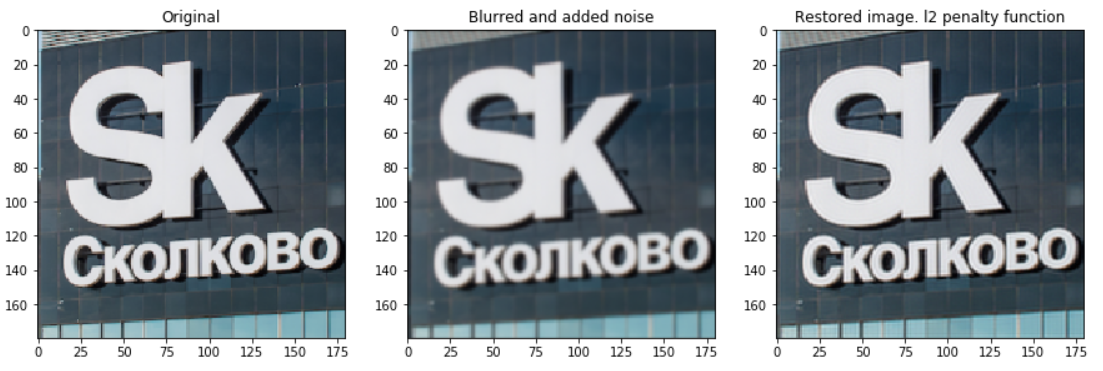
\includegraphics[scale=0.37]{grad_l2_small.png} \\
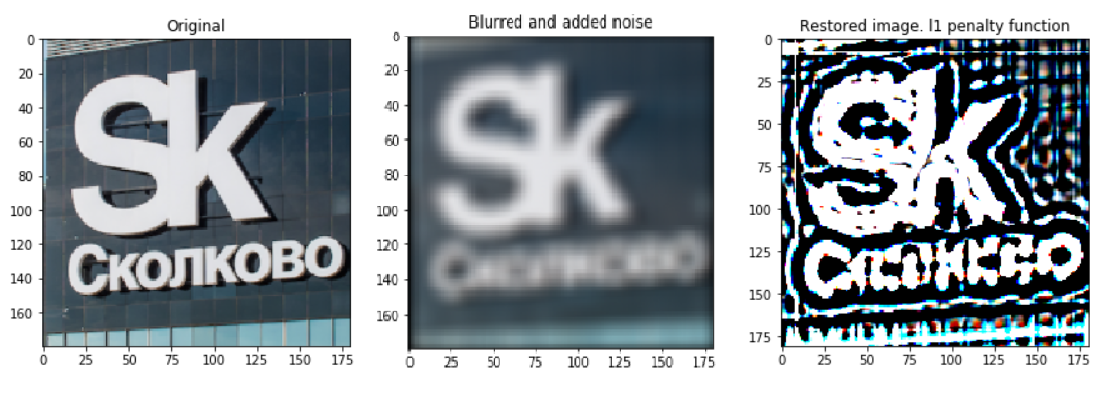
\includegraphics[scale=0.37]{grad_l1_big.png} \\
\end{adjustwidth}
\caption{.}
\end{figure}
\end{center}

\end{frame}
%------------------------------------------------------------------------------
\subsection{Proxi Gradient}
\begin{frame}
\frametitle{Proxi Gradient. Kernel = (4, 4)}
\begin{center}
\begin{figure}[h]
\begin{adjustwidth}{-0.2cm}{-0.5 cm}
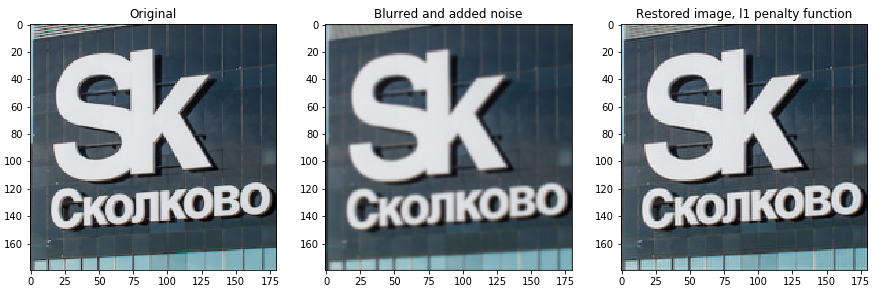
\includegraphics[scale=0.355]{l1_all_imgs_4_4.png} \\
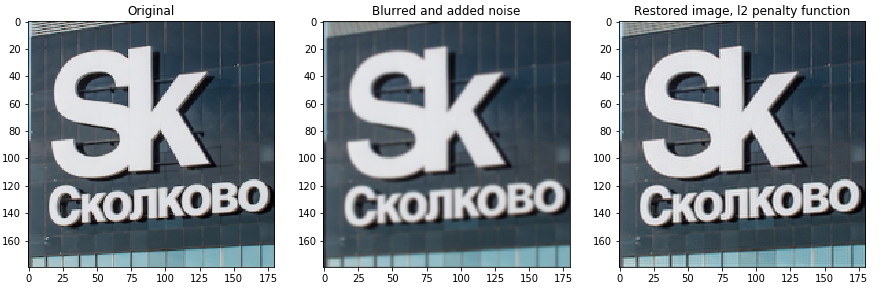
\includegraphics[scale=0.355]{l2_all_imgs_4_4.png} \\
\end{adjustwidth}
\caption{.}
\end{figure}
\end{center}

\end{frame}
%------------------------------------------------------------------------------
\begin{frame}
\frametitle{Proxi Gradient. Kernel = (3, 15)}
\begin{center}
\begin{figure}[h]
\begin{adjustwidth}{-0.2cm}{-0.5 cm}
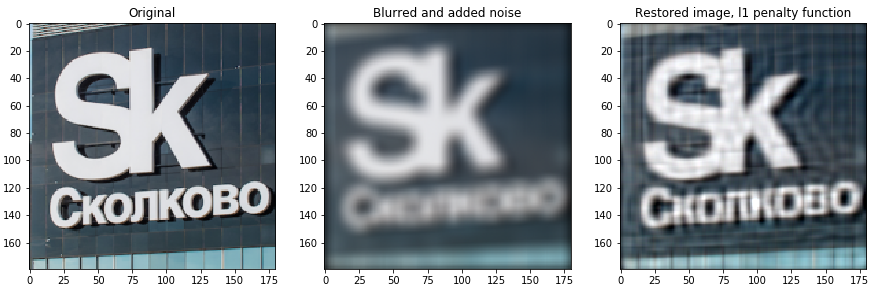
\includegraphics[scale=0.355]{l1_all_imgs_3_15.png} \\
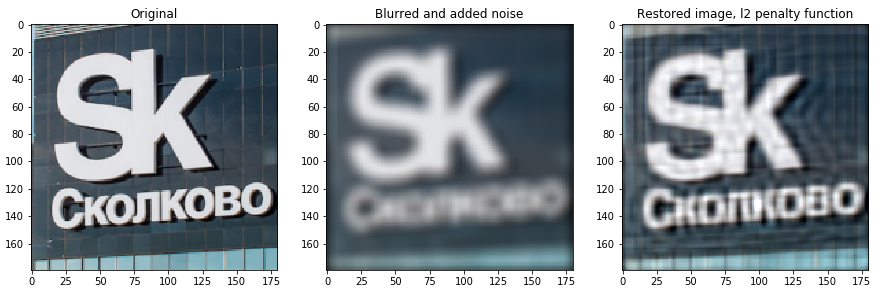
\includegraphics[scale=0.355]{l2_all_imgs_3_15.png} \\
\end{adjustwidth}
\caption{.}
\end{figure}
\end{center}

\end{frame}
%------------------------------------------------------------------------------
\subsection{Newton Method}
\begin{frame}
\frametitle{Newton Method. Different initializations}

\begin{center}
\begin{figure}[h]
\begin{adjustwidth}{-0.9cm}{-0.9 cm}
\begin{tabular}{cc}
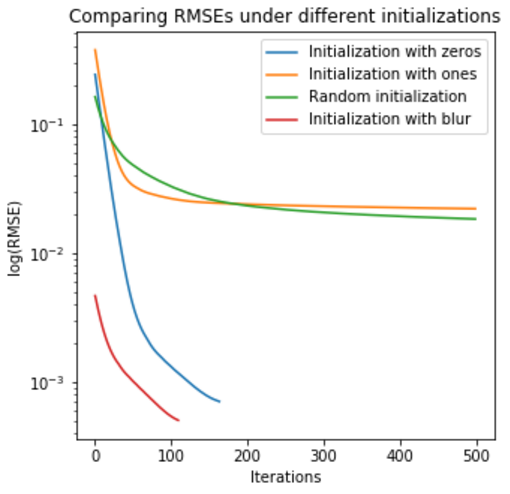
\includegraphics[scale=0.435]{new_rmse.png} &
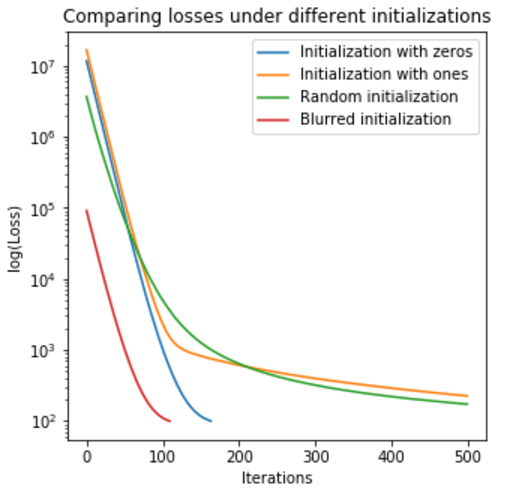
\includegraphics[scale=0.435]{new_loss.png} 
\end{tabular}
\end{adjustwidth}
\caption{.}
\end{figure}
\end{center}
\end{frame}
%------------------------------------------------------------------------------
\begin{frame}
\frametitle{Newton Method. Kernel = (4, 4)}

\begin{center}
\begin{figure}[h]
\begin{adjustwidth}{-0.2cm}{-0.5 cm}
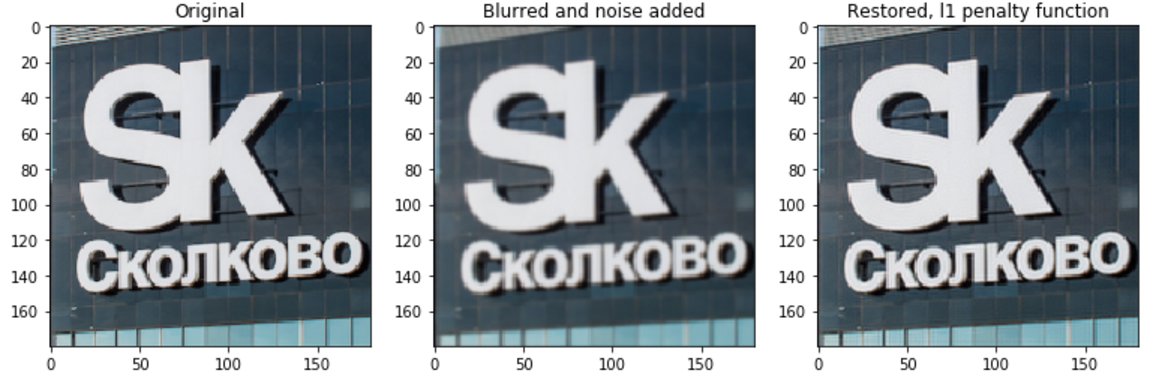
\includegraphics[scale=0.27]{new_small_l1.png} \\
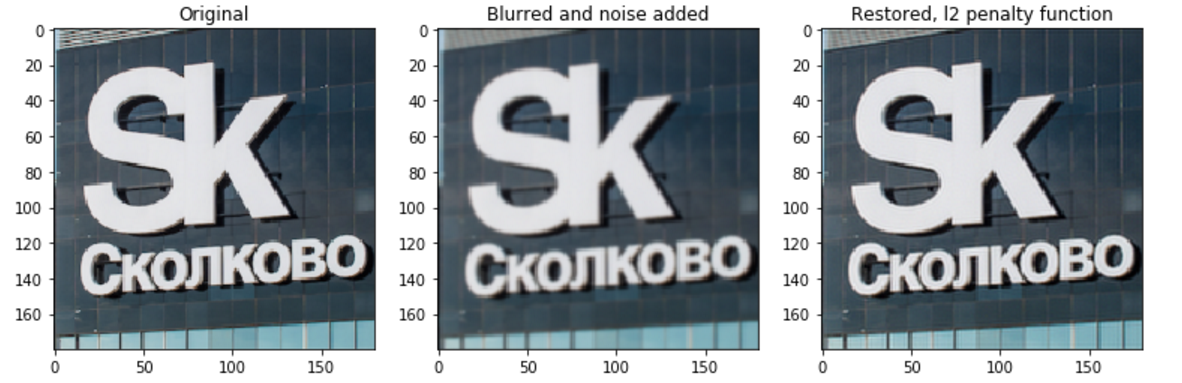
\includegraphics[scale=0.27]{new_small_l2.png} \\
\end{adjustwidth}
\caption{.}
\end{figure}
\end{center}

\end{frame}
%------------------------------------------------------------------------------
\begin{frame}
\frametitle{Newton Method. Kernel = (3, 15)}

\begin{center}
\begin{figure}[h]
\begin{adjustwidth}{-0.2cm}{-0.5 cm}
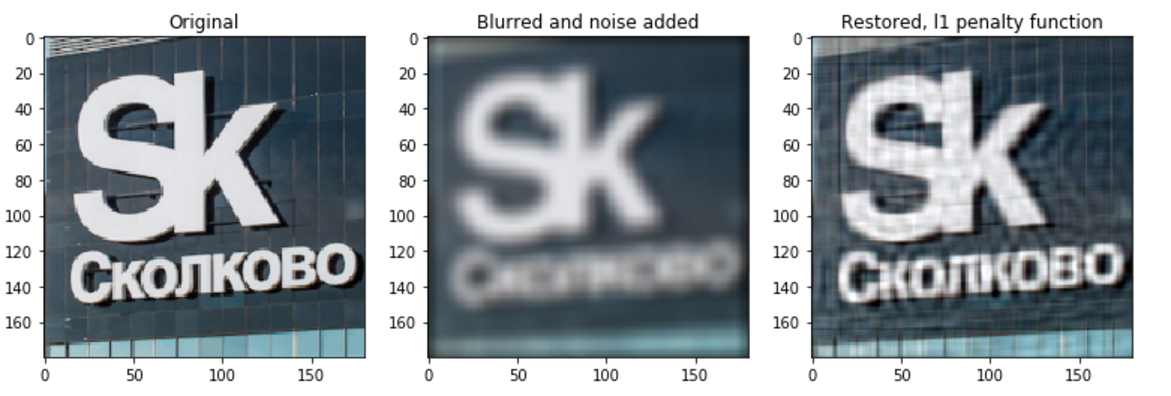
\includegraphics[scale=0.27]{new_big_l1.png} \\
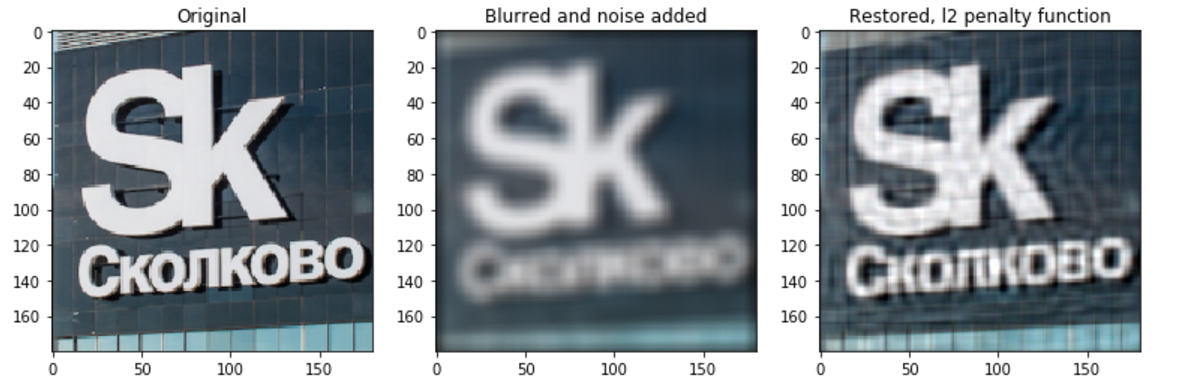
\includegraphics[scale=0.27]{new_big_l2.png} \\
\end{adjustwidth}
\caption{.}
\end{figure}
\end{center}

\end{frame}
%------------------------------------------------------------------------------
\section{Conclusion} 
\subsection{RMSE Rate}
\begin{frame}
\frametitle{RMSE Rate. Kernel = (4, 4)}

\begin{center}
\begin{figure}[h]
\begin{adjustwidth}{-0.3cm}{0.9 cm}
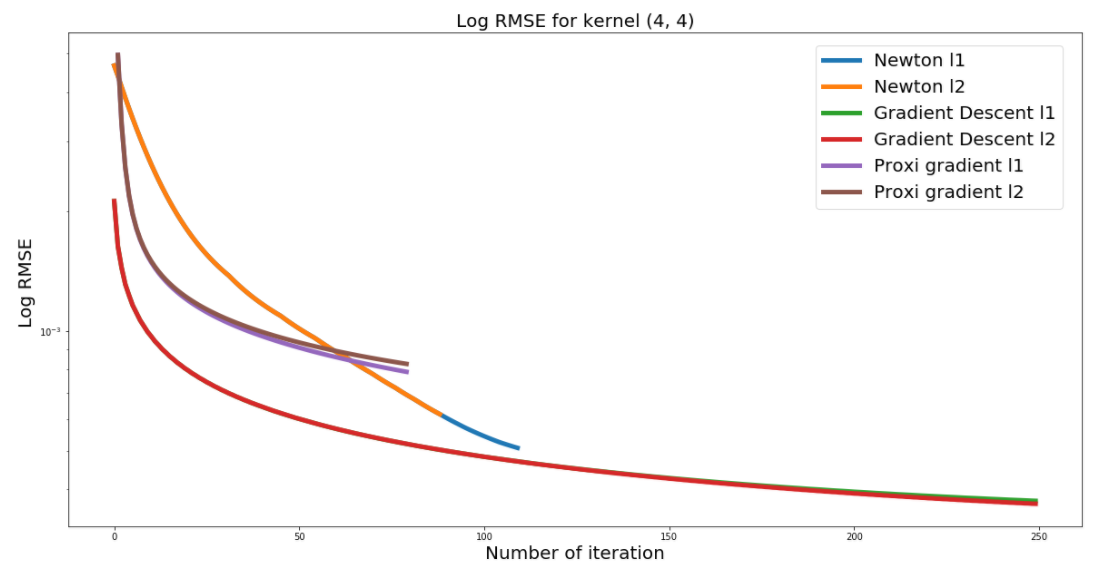
\includegraphics[scale=0.4]{rmse_small.png}
\end{adjustwidth}
\caption{.}
\end{figure}
\end{center}

\end{frame}
%------------------------------------------------------------------------------
\begin{frame}
\frametitle{RMSE Rate. Kernel = (3, 15)}

\begin{center}
\begin{figure}[h]
\begin{adjustwidth}{-0.3cm}{0.9 cm}
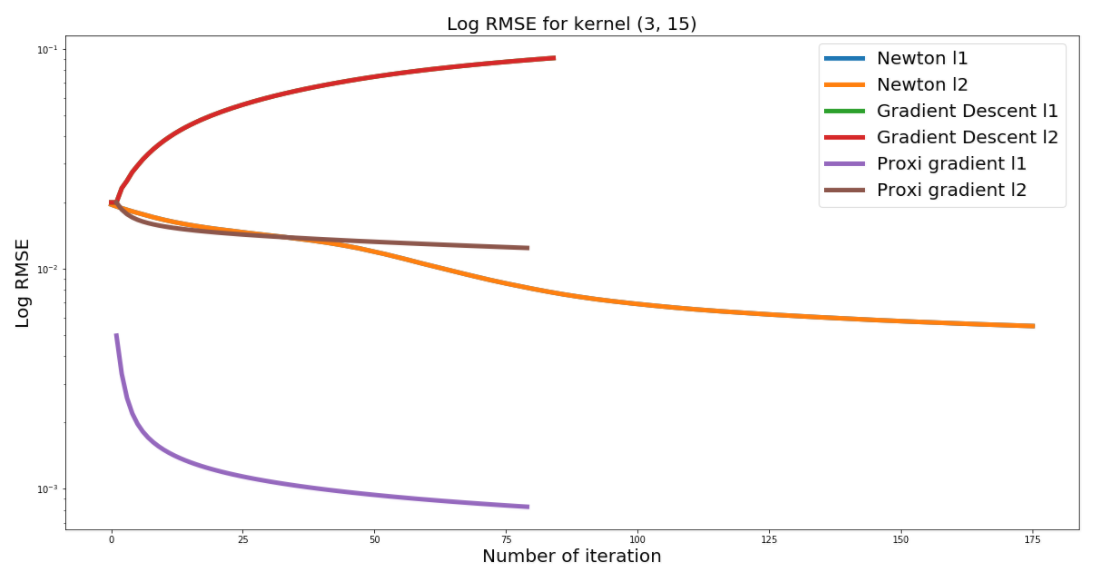
\includegraphics[scale=0.4]{rmse_big.png}
\end{adjustwidth}
\caption{.}
\end{figure}
\end{center}

\end{frame}
%------------------------------------------------------------------------------
\subsection{Loss Rate}
\begin{frame}
\frametitle{Loss Rate, Kernel = (4, 4)}

\begin{center}
\begin{figure}[h]
\begin{adjustwidth}{-0.3cm}{0.9 cm}
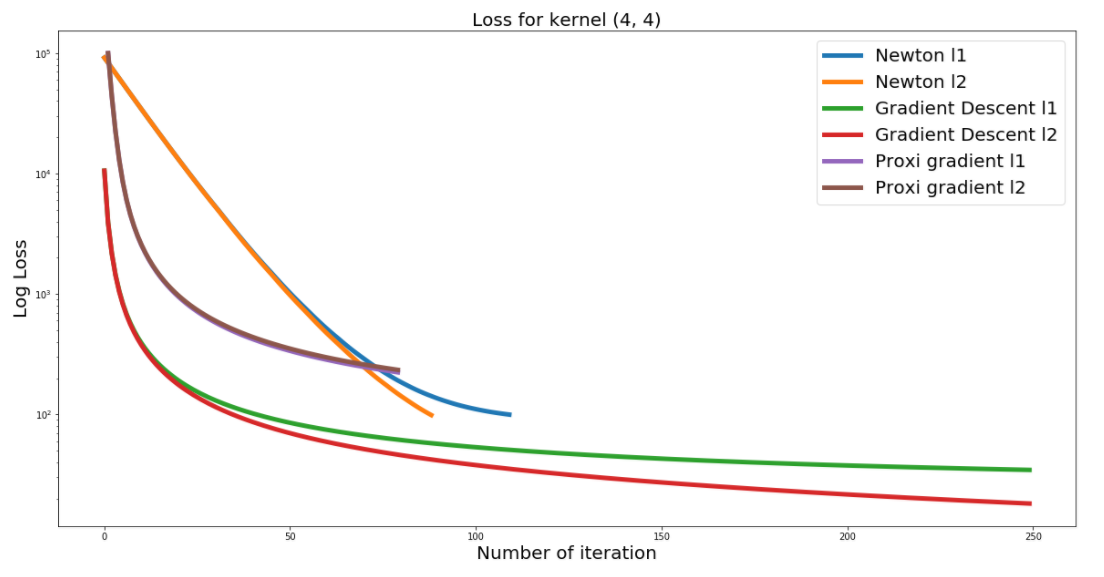
\includegraphics[scale=0.4]{loss_small.png}
\end{adjustwidth}
\caption{.}
\end{figure}
\end{center}

\end{frame}
%------------------------------------------------------------------------------
\begin{frame}
\frametitle{Loss Rate, Kernel = (3, 15)}

\begin{figure}[h]
\begin{adjustwidth}{-0.5cm}{-0.9 cm}
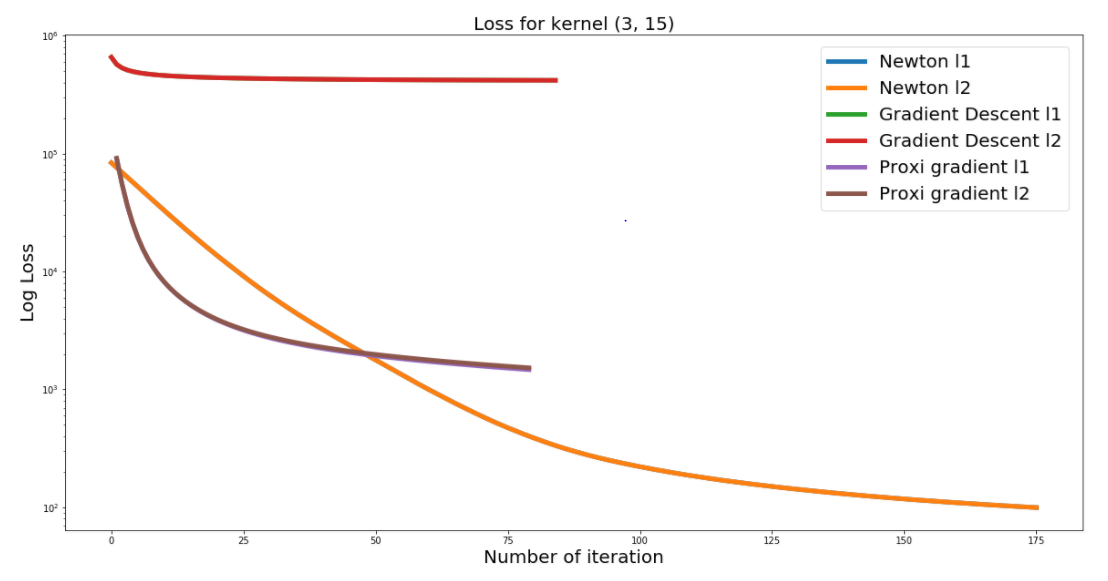
\includegraphics[scale=0.4]{loss_big.png}
\end{adjustwidth}
\caption{.}
\end{figure}

\end{frame}
%------------------------------------------------------------------------------
\subsection{Conclusion}
\begin{frame}
\frametitle{Final comparison}

\begin{table}
\centering\medskip\tabcolsep6pt
\begin{tabular}{|c||c|c|c|c||}
\hline
& \multicolumn{4}{c||}{Kernel(4, 4)} \\
\hline
 & RMSE, l1 & RMSE, l2 & Loss, l1 & Loss, l2 \\	
\hline
CVXPY &  0.063  & 0.058  & 48.094  & 5.302   \\
\hline
Fast Gradient & 0.0007 & 0.0007 & 159.129 & 143.742  \\
\hline
Proxi Gradient & 0.0004 & 0.0005 & 88.271 & 94.285  \\
\hline
Newton method & 0.0005 & 0.0006 & 99.680 & 98.794  \\
\hline
\end{tabular}
\end{table}

\begin{table}
\centering\medskip\tabcolsep=6pt
\begin{tabular}{|c||c|c|c|c||}
\hline
& \multicolumn{4}{c||}{Kernel(3, 15)} \\
\hline
 & RMSE, l1 & RMSE, l2 & Loss, l1 & Loss, l2 \\	
\hline
CVXPY & 0.305  & 0.304  &  2392 & 1906  \\
\hline
Fast Gradient & 0.126 & 0.126 & 412988 & 412949  \\
\hline
Proxi Gradient & 0.008 & 0.009 & 373.271 & 510.558 \\
\hline
Newton method & 0.005 & 0.005 & 99.957 & 99.654  \\
\hline
\end{tabular}
\end{table}

\end{frame}

%------------------------------------------------------------------------------
\begin{frame}
\frametitle{Conclusions}

\begin{itemize}
\item Problem formulated 
\item Different approaches for solving were studied
\item Data prepared
\item Software developed, variations considered
\item Results compared
\item Team work appreciated
\end{itemize}

\end{frame}

%------------------------------------------------------------------------------
\subsection{Team}
\begin{frame}
\frametitle{Our Team}

\begin{figure}[h]
\begin{adjustwidth}{-1.1cm}{-0.9 cm}
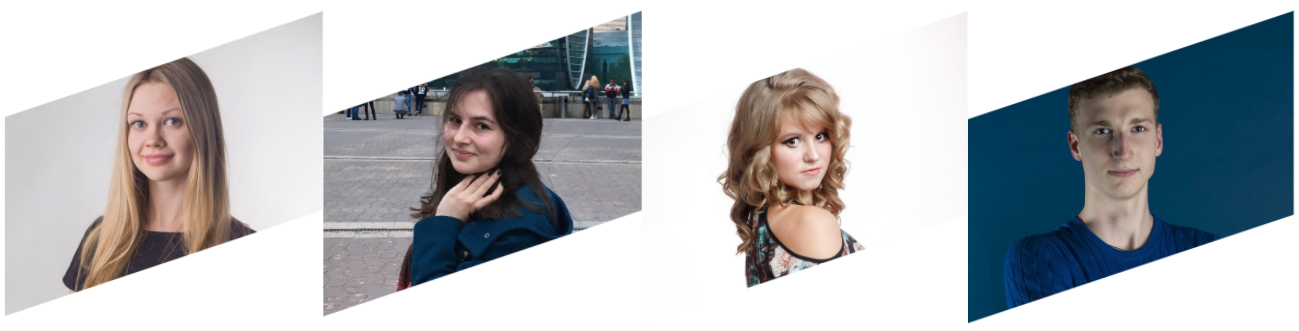
\includegraphics[scale=0.38]{Team.png}\\
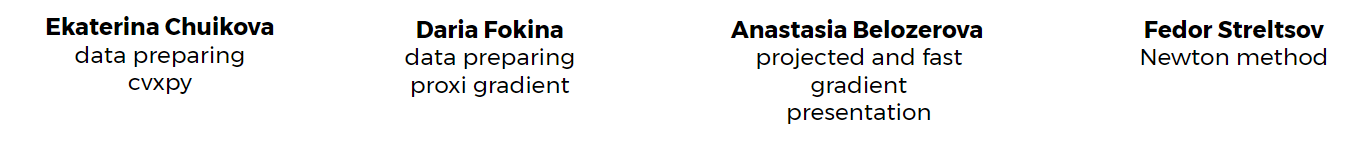
\includegraphics[scale=0.35]{signs.png}
\end{adjustwidth}
\caption{.}
\end{figure}

\end{frame}

%------------------------------------------------------------------------------
\end{document}
